

\textbf{text gras}\hfill \\ \indent text indent�

%cf wikibook font size
\Large{}\normalsize
\LARGE{}\normalsize
\huge
\Huge


\footnote{Source : \url{}}

%Ne pas mettre de caract�res accentu�s dans les titres ci-dessous
\chapter{chapX}\label{chapter:chapX}
\section{section}
\subsection{sous-section}
\subsubsection{sous-sous-section}


une ligne\\ une ligne � la ligne

\c{c} : �
\'{e} : �
\`{e} : �
\`{a} : �
\^{a} : �
\^{e} : �
\"{e} : �
\oe{}
\{
\%
\_
\textbackslash{}


\textquote{derri�re}


1\up{er}

%Juste une liste
\begin{itemize}
	\item un �l�ment de liste\index{ref pour l'index}
\end{itemize}
%
\begin{description}
	\item[un titre en gras] \hfill \\
	une description indent�e

\end{description}



%%IMAGES
\ref{figure:} page \pageref{figure:}

\begin{figure}[!h]% h || ht || .... cf 
  \centering
      \includegraphics[width=\textwidth+1cm,height=\textheight-1.5cm]{images/.jpg}
  \caption{}
	\label{figure:}
\end{figure}


%% PDF
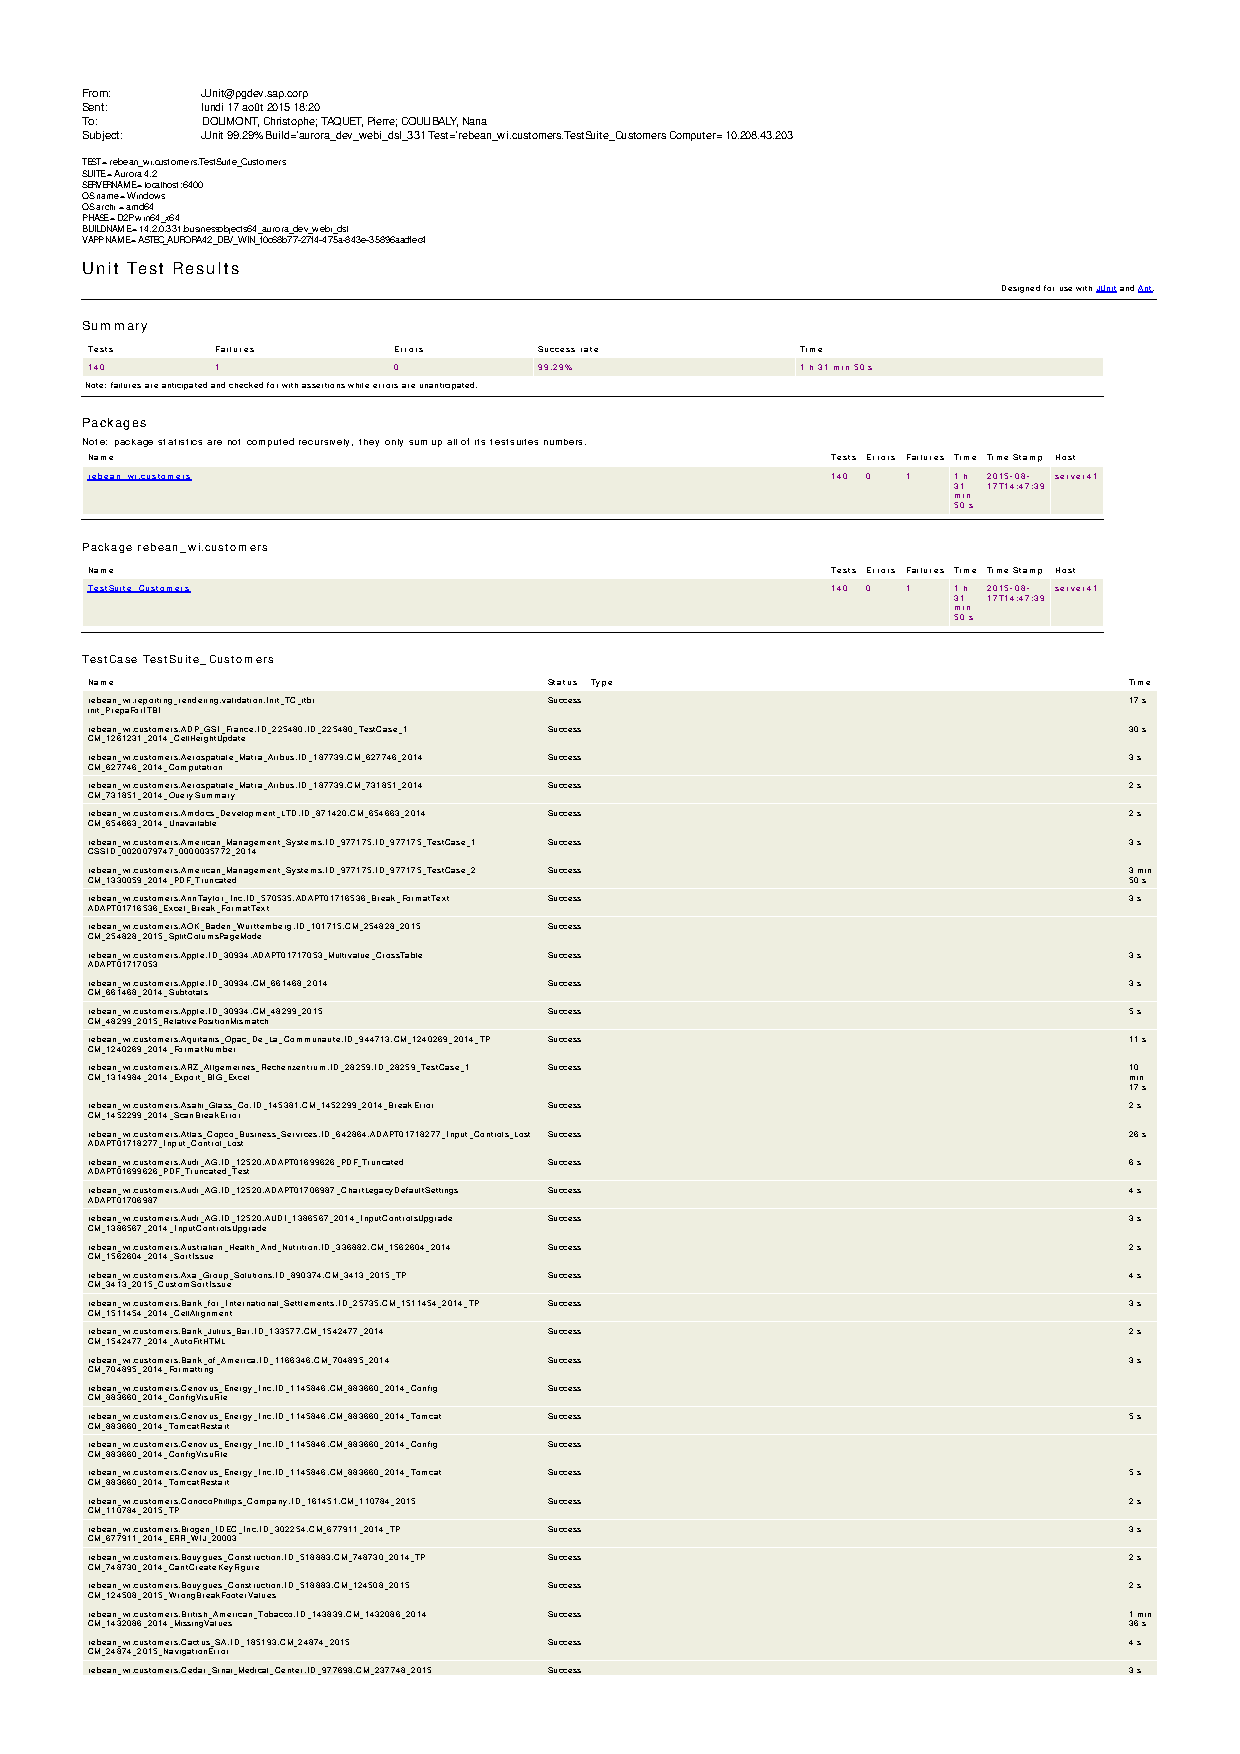
\includepdf[pages=-,scale=0.9,pagecommand={}\label{pdf:org}]{images/AutomationResults.pdf}

%%% adapt geometry
%% 0 partout et sa "supprime" header footer etc qui se retrouvent � l'ext�rieur
\newgeometry{left=1cm,right=1cm,top=0cm,bottom=2cm}
\restoregeometry

%Ins�rer du code
%Attention � la config n�cessaire !
\lstinputlisting[language=java]{scripts/basicStaticTest.java}

% Pour les longs mots, ceux-ci se retrouvent coup�s si c'est d�conn�
\begin{sloppypar}
\end{sloppypar}

%plus simple mais verbeux
\begin{lstlisting}
MonoDocTestCase(MonoDocTestCaseConfigInfo tccInfo, String sDocumentName, String sCategoryType, String sCategory, Boolean useAuroraCtx);
\end{lstlisting}


\url{https://url}


%% TABLE
\begin{tabular}{|l|c|r|}
  \hline
  colonne 1 & colonne 2 & colonne 3 \\
  \hline
  1.1 & 1.2 & 1.3 \\
  2.1 & 2.2 & 2.3 \\
  \hline
\end{tabular}


\begin{table}[h!]
	\begin{center}
     \begin{tabular}{ c  p{5cm}  p{5cm}  }
			 \toprule
				my.Lboro & Advantages & Disadvantages \\ 
			\cmidrule(r){1-1}\cmidrule(lr){2-2}\cmidrule(l){3-3}
			 \raisebox{-\totalheight}{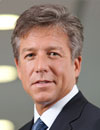
\includegraphics[width=0.3\textwidth, height=50mm]{images/sap-executive-mcdermott.jpg}}
				& 
				\begin{itemize}[topsep=0pt]
				\item Accessibility
				\item Up to date information
				\item Fulfil students needs and wants \ldots
				\end{itemize}
				& 
				\begin{itemize}[topsep=0pt]
				\item Accessibility
				\item Up to date information
				\item Fulfil students needs and wants \ldots
				\end{itemize}
				\\ 
				
				\bottomrule
				\end{tabular}
		\caption{my.Lboro Analysis}
		\label{tbl:myLboro}
	\end{center}
\end{table}





\usepackage{textcomp}%  \texttildelow